\documentclass[12pt]{article}


\usepackage{charter}
\usepackage{fullpage}
\usepackage[colorlinks=false,unicode]{hyperref}
\usepackage{ifthen}
\usepackage{comment}
\usepackage[title,titletoc]{appendix}
\usepackage{pagecolor}
\usepackage{amsmath}
\usepackage{amsfonts}
%\usepackage[normalem]{ulem}
\usepackage{siunitx}
\usepackage{amsthm}
\sisetup{per=slash, load=abbr}

\usepackage{pgfplots}
\usetikzlibrary{positioning}
\usetikzlibrary{fit}
\usetikzlibrary{snakes}
\usetikzlibrary{shapes.geometric}
\usetikzlibrary{patterns}
\usetikzlibrary{shapes,arrows,chains}
\usepgfplotslibrary{patchplots,colormaps}
\usetikzlibrary{calc}
\usetikzlibrary{positioning, fit}
\usetikzlibrary{backgrounds}
\usetikzlibrary{intersections}

\newcommand{\whitepaper}[1]{\begin{center}\fbox{\parbox{0.95\textwidth}{{\footnotesize
#1}}}\end{center}}

\newcommand{\pcolor}{orange!25}

\usepackage{setspace}
\usepackage{algorithm2e}
\bibliographystyle{ieeetr}

\usepackage{geometry}
\geometry{left=3cm,right=3cm,top=1.6cm,bottom=3cm,headheight=0pt,headsep=1.5em}
\usepackage{fancyhdr}
\pagestyle{fancy}
\chead{
\includegraphics[scale=0.1]{../common/Nebulas.png}}  %在此处插入logo.pdf图片 图片靠左
\lhead{} % 页眉中间位置内容
\rhead{}
%\setlength{\topskip}{1em}

\usepackage{enumerate}
\setcounter{tocdepth}{4}
\setcounter{secnumdepth}{4}


\usepackage{indentfirst}


\newcommand{\reffig}[1]{Fig.~\ref{#1}}
\newcommand{\refeq}[1]{Equation~\ref{#1}}
\newcommand{\refsec}[1]{~\S~\ref{#1}}


%\setlength{\parindent}{2.1em}
%\setlength{\parskip}{0.3\baselineskip}
\newcommand{\nrcore}{Core Nebulas Rank}
\newcommand{\nrext}{Extended Nebulas Ranks}
\newcommand{\nr}{Nebulas Rank}
\newcommand{\dom}{{\; \texttt{dom}\;}}

\onehalfspacing

\newtheorem{property}{Property}
%\addbibresource{reference.bib}

\begin{document}
\pagestyle{empty}
%\renewcommand{\nomname}{术语表(按首字母排序)}
%\renewcommand{\baselinestretch}{1.5}

%\pagecolor{\pcolor}

\begin{titlepage}
  \begin{center}
    \vspace*{5.5cm}
    
\includegraphics[scale=0.4]{../common/Nebulas.png}
    \vspace{0.5cm}


    \textbf{\huge{White Paper}}

    \vspace{0.5cm}
    Zhuoer Wang \\
    Translate: Dustin Kritzer
    \vfill
    July 2019\\
    Version: 0.0.1
    \textbf{}
  \end{center}

\end{titlepage}
\setcounter{page}{0}
%\thispagestyle{empty}
\tableofcontents
\newpage
\setcounter{page}{1}
\pagestyle{fancy}
\vspace*{0.01cm}
% !TEX root = main.tex
\section{概述}

\textbf{关键字: Token Economy\ 经济体\ 去中心化\ 协作\ 激励\ 自进化\ 自治 }

\vspace{2em}

星云链(Nebulas)是开源公链,星云是\textbf{自治元网络}(Autonomous Metanet)~\cite{AutonomousMetanet},星云专注于处理复杂数据和交互、复杂的协作关系,致力于通过区块链等技术手段,实现让每个人从去中心化协作中公平获益的愿景~\cite{vision}。

NAX是质押币。

全新智能资产平台nextDAO致力于构建更好的去中心化自治组织,更好的Token经济(Better DAO, Better Token Economy),关注链上互动和协作,提供去中心化金融工具,重新定义Token经济,发现新的业务场景,推动生态应用落地。从星云生态起步,核心技术沉淀到星云链主网,鼓励从模式到范式的创新,最终形成通用模块,为更广泛的用户所用。
\section{背景介绍}

其中,“NAT 链上投票”是核心手段,包括两部分:
1. 投票唯一介质:NAT 及其底层算法是星云链上治理的重要工具;
2. 链上投票流程。
本章节将对其进行重点介绍。
12
5.2 投票基本原则
星云生态通过星云主网实现链上投票。社区投出的每一票,将在星云链的区块上
公开透明地展现。在星云链的系统中,投票将遵循以下基本原则:
1. 投票的最基本单位是一个星云主网地址。
2. 星云链的投票权重将参照地址的星云指数。
3. 对系统有积极贡献的行为应被奖励更多的投票权,在投票的场景中,我们认为
投票行为是对星云系统有积极贡献的行为,应被激励更多的投票权。
5.3 投票方式
投票将通过星云主网上的投票智能合约实现,每个地址可以选择投赞同、反对、
弃权三种票。亦可不参与投票。
5.4 投票唯一介质:NAT
5.4.1 概述
• 名称: Nebulas Autonomous Token
• 代号: NAT
• 形式: NRC20 token
NAT 是星云指数的资产形态,它以NRC20 Token 的形式体现,并作为星云生态
治理场景中唯一的投票介质。


作为社区治理币,需要明确几个设计目标,最终NAX设计出来需要达到哪些目标。在确定一个系列目标的基础上,再进行机制的设计,所有机制的设计也将需要符合这个总的目标。为了使得机制设计简洁、清晰,一切与目标不相关的设计,都不应该随意纳入机制当中,以妨止最终偏离初衷。以下是几点关于治理币几个总的目标:

\begin{enumerate}[a.]
        \item 用于星云社区治理
        \item 星云社区贡献有效凭证
        \item NAX需要是符合通缩模型
        \item NAX有升值空间
        \item 销毁与增发达到一定程度的平衡
\end{enumerate}

星云治理的目的是实现星云愿景,聚焦去中心化协作。在谈论具体的星云治理措施之前,需要先了解当前新场景下出现的协作困境,以及星云的治理方式想要解决的问题。

\label{background}

人类是具有社会性的,我们对协作(Collaboration)并不陌生。即便是孤岛上的鲁滨逊,也和星期五磨合出了一套相处模式~\cite{robinson}。协作方式本身没有绝对高低优劣之分,在不同场景下,应选择适合该场景的一种或多种协作方式。随着科技的发展,协作场景已经从人与人面对面合作,升级到全球化的跨越多地区、并有多组织参与的协作。协作的目标结果也更为多变,成果从实物到虚拟,协作的时间跨度也变得更长、更灵活。

星云并不力求颠覆其它协作方式,也不排斥多种协作方式混用。星云尝试寻找更合适的协作方式,补足当前其它协作方式在新场景下的不足。新的应用场景有如下特点:

\begin{itemize}
	\item \textbf{信息交互从单⼀、简单的功能向复杂、多样发展。}
	
	去中心化的电子加密货币比特币的诞生让区块链可以记录交易信息。以以太坊为代表的第二代区块链系统提出了具有图灵完备性的智能合约,区块链变得可编程。逐步出现了链内、链外、“跨链”等不同场景的数据和资产交互问题。

	\item \textbf{用户角色也随之越来越多。}

	早期比特币社区只有矿工和持币者,有了以太坊之后出现了开发者、应用使用者等,越来越多的人接触到区块链,不同用户角色的责权利如何分配受到挑战。

\end{itemize}

当前常见的协作方式在新场景下的不足举例:

\begin{enumerate}
	\item 

	\textbf{中心化治理无法应对复杂的新场景。}

	区块链技术本质上是⼀种去中心化、⾮信任、基于博弈的⾃治体系,其真正的魅力是在去中⼼化思想下,基于共识机制的开放协作模式~\cite{whitepaper}。但有的区块链项目干脆反其道而行之,使用中心化方式进行治理,如直接通过核心仲裁法庭直接对黑客进行判决。这种方式的正当性和公平性难以得到保障。面对复杂的数据交互形态和丰富的用户角色,中心化的单一评判标准很难做到广而全面,引起社区成员反抗。2019年1月11日,EOS Authority发起了关于是否废除ECAF(EOS核心仲裁法庭)的投票,支持废除的比例高达98\%~\cite{DeleteECAF}。

	\item 

	\textbf{现有的去中心化治理方式规则不统一。}

	例如比特币社区,对矿工和持币者等不同角色的用户来说,对应的规则并不相同,且不明确。此类去中心化治理方式容易引起社区发展目标不明确,难以有效组织和迭代升级。

	\item 

	\textbf{传统去中心化协作方式常现公地悲剧~\cite{TragedyOfTheCommons}。}

	传统去中心化协作项目,如大量开源社区,本身利益模型不明确,经费来源往往主要靠捐赠,升级进化过于依赖开发者的兴趣,经常会出现公地悲剧、生态进化缓慢等问题。使用公共资源(如开源代码)的人多,作出贡献的人少。依托大公司和企业定向捐赠的开源项目又经常会被大公司的发展方向牵制,成为企业的附属。

	区块链技术因为有了代币的存在,让我们有机会通过提供可持续的激励,构建良性经济体来解决去中心化协作的基本困境。

	\item

	\textbf{早期区块链项目共识机制激励不全面,社区参与度低。}

	如比特币使用的共识机制工作量证明(Proof of Work,PoW~\cite{pow})仅专注挖矿激励,此种单一激励不能应对用户角色的逐渐丰富。去中心化的以太坊由于升级缓慢而饱受诟病。以太坊的升级提案需要得到社区广泛认同后由矿工完成操作之后才可执行,但整个生态中各方意见难以统一,以太坊的激励没有覆盖整个生态的不同用户角色。“事不关己”的现象导致以太坊升级提案参与度低,迟迟难以执行,生态发展受阻。

\end{enumerate}

目前不存在完善的方案可以解决上述问题。我们意识到,应对具备前所未有复杂度的新世界,新技术的诞生众望所归。


\section{设计原则}

根据费雪公式:
\begin{equation}
M * V = T / P
\end{equation}
\(M\)是Token数量,\(V\)是Token流通速度,\(P\)是Token价格,而\(T\)是系统内总交易额。很好理解,等式两边其实算的都是以Token数量为计量的GDP。左边\(M * V\)是个数乘以流通速度等于GDP(Token计量),右边总GDP(法币计量)除以Token价格(法币计量)也等于GDP(Token计量)。

通过这个公式,我们不难推出(以后补上推理步骤)通过增加持币价值是最终有效的提升币价和使用价值的方式。

\subsection{减少NAS流通量}
\subsubsection{增加质押}
\subsubsection{增加地址数}
\subsubsection{减少交易所存量}
\subsection{增加持有NAS和NAX的动力(减少交易动力)}
\subsection{增加NAX使用和消耗场景 (供需平衡)}

\section{Organization and Supervision: Nebulas Community Group}

In order to achieve the goal of ecological development as well as asset management and to support Nebulas' goal of creating the Autonomous Metanet, the founding team will form the \textbf{Nebulas Community Group} together with the community. During the formation process, each organization's source of legitimacy, power, and boundaries will be strictly stipulated and constrained by one another. The three major organizations that comprise the Nebulas Community Group are:

\begin{enumerate}
	\item \textbf{Nebulas Council}: Oversees the legitimacy of the Nebulas governance process and the use of public assets within the Nebulas community; providing scaling advantages for the ecological development of Nebulas.
	\item \textbf{Nebulas Foundation}: Manage the Nebulas Foundation's public assets, pool available resources and use the capital to offer efficiency advantages to the Nebulas ecosystem.
	\item \textbf{Nebulas Technical Committee}: Entrusted by the Nebulas Council; responsible for the productivity and quality verification of development projects as well as providing technical guidance and support to the community.
\end{enumerate}

\vspace{2em}

To ensure the independence of the Nebulas Community Group and to maintain checks and balances between them, there are two fundamental requirements:

\begin{enumerate}
	\item \textbf{The restraint of personal power}: All organizations are open to participants within the Nebulas community; however, a community member cannot hold a position in more than two organizations at the same time.
	\item \textbf{The restraint of organization power}: No single organization has the power to make independent decisions and to use public assets without the oversight of the other organizations.
\end{enumerate}

If it's necessary to introduce new principles, the three organizations must always be guaranteed independent operation and to be constrained by one another.

\subsection{Nebulas Council}

The Nebulas Council oversees the Nebulas governance process and the use of public assets of the Nebulas community to provide scale advantages for further ecological development of Nebulas.

\subsubsection{Directors}

The first directors of the Nebulas Council will comprise of 7 seats; of which, 3 seats will be nominated by the Nebulas Foundation and 4 seats will be elected via on-chain public voting within the community.

The numbers of nominations from the Nebulas Foundation are reduced by at least one seat every two years. After 6 years, the Nebulas Foundation can no longer nominate seats.

\subsubsection{Power}

\begin{enumerate}
	\item The Nebulas Council has the power to submit a proposal for a \textbf{second vote} (\ref{second-vote}).
	\item Appoint organizations such as the Nebulas Technical Committee or individuals to handle public affairs for the Nebulas community.
\end{enumerate}

\subsubsection{Obligations}

\begin{enumerate}
	\item Supervise the governance process.
	\item Supervise the safety of public assets such as community reserve funds.
\end{enumerate}

The Nebulas Council should ensure that the governance processes and the use of community public property are open and transparent. These methods include but are not limited to:

\begin{enumerate}
	\item Regularly updated asset use and community development via quarterly reports and other disclosure materials to the communities.
	\item Any technical upgrade, project application rejection, re-voting, etc. should be announced in a timely manner.
	\item All personnel elections and appointments should be announced on time.
\end{enumerate}

\subsubsection{Term of office}

The directors of the Nebulas Council have a term of two years and can be re-elected once their term is over.

\vspace{2em}


Community members have full oversight of the Nebulas Council. The directors of the Nebulas Council must comprise a report of their duties for their full term. The community will conduct a mid-term vote based on the submitted report to determine whether each Nebulas Council director will continue to serve.

If the director of the Nebulas Council fails to pass the midterm vote, the Nebulas Technical Committee will organize and supervise the election of a replacement Nebulas Council director. The directors who passed the mid-term review will temporarily complete the daily affairs of any directors who were removed until the election of the new Nebulas Council director is completed.

\subsubsection{Election method}

Except for the directors of the Nebulas Council nominated by the Nebulas Foundation, the directors of the Nebulas Council are elected through public on-chain voting. All members of the community who control at least one address on the Nebulas mainnet have the right to vote and to run for a seat on the council.

The first Nebulas Council election program has been proposed and will be supervised by the Nebulas Foundation. Future changes and iterations of the process must be performed through public, on-chain voting.

\subsubsection{Income}

\textbf{Total revenue}

10,000 NAS distributed over the 2-year term as described below.

\vspace{2em}

\textbf{Income distribution}

The revenue will be issued once every six months (four times in two years). The amount of each distribution every 6 months in order is: 1,500 NAS, 2,000 NAS, 3,000 NAS, 3,500 NAS (totaling 10,000 NAS). If the mid-term vote is not passed, the latter two payment will not be released.

\vspace{2em}

\textbf{Financial requirements}

To ensure the best interests of the economy and the continuity of the Nebulas Council, directors of the Nebulas Council must deposit 100,000 NAS into collateral for the initial 6 months of their term.

\vspace{2em}

\subsection{Nebulas Foundation}

The Nebulas founding team was formed in June of 2017; later, the Nebulas Foundation was established to take charge of the Nebulas team, their financial options, to ensure the normal operation of the project and to realize the development roadmap as promised in the \textit{Nebulas Non-technical Whitepaper}.

After all the technical points in the Nebulas Non-technicaal Whitepaper are fully completed, the Nebulas Foundation will manage the Foundation’s assets, pool resources, and use the capital to provide efficiency advantages for the ecological development of Nebulas.

\subsubsection{Members composition}

The managing directors of the Nebulas Foundation have no less than 5 seats including one chairman of the Nebulas foundation and one chief secretary.

\subsubsection{Power}

\begin{enumerate}
	\item Participate in the election of the chairman as well as the right to be elected.
	\item Participate in decision making in items such as foundation development and investment.
\end{enumerate}

\subsubsection{Obligations}

\begin{enumerate}
	\item Manage the assets and pool resources of the Nebulas Foundation.
	\item According to the needs of Nebulas, ensure the research and development of Nebulas and complete the technical features as promised in the Nebulas non-technical Whitepaper on time.
	\item Once a year, Nebulas Foundation directors will report to the Nebulas Council and continue to serve the Nebulas ecosystem.
\end{enumerate}

\subsubsection{Term in office}

The members of the Nebulas Foundation are appointed for a one year term. Afterwards, they are eligible for re-election.

\subsubsection{Inclusion method}

\textbf{Inclusion method}

The Nebulas Foundation adopts a capital-based entry system and all who receive the financial option reward to a certain amount are automatically eligible to become a Foundation Managing Director. Subsequently, all eligible members have the option to waive becoming a Foundation Managing Director. If there are less than 5 members within the Board of Managing Directors, they will be ranked according to their financial option reward size.

\vspace{2em}

\textbf{Chairman of the Nebulas Foundation}

The chairman of the Nebulas Foundation is elected among the current members of the Nebulas Foundation. Each member of the Nebulas Foundation has the right to vote and to be elected.

To become the chairman of the Nebulas Foundation, a member must receive a minimum of 50\% of all casted votes. During voting and none of the directors receive 50\% of the votes, those with either no votes or the minimum amount of votes are eliminated and voting will be restarted until a member receives an approval rating of 50\% or greater.

\vspace{2em}

\textbf{Chief Secretary of the Nebulas Foundation}

The Chief Secretary of the Nebulas Foundation is appointed by the Chairman of the Nebulas Foundation among current members of the Nebulas Foundation.

\vspace{2em}

\textbf{Managing Director of the Nebulas Foundation}

The Managing Director of the Nebulas Foundation is appointed by the Chairman among current members of the Nebulas Foundation.

\vspace{2em}

\textbf{Recall}

The Nebulas Foundation can remove any member of the Nebulas Foundation through internal resolutions and the results must be disclosed to the community.

The removed member(s) of the Nebulas Foundation has the right to address to the community publicly and call for a public, on-chain vote to request a re-vote for reinstatement to the Foundation.

\subsubsection{Income}

\textbf{Total revenue}

\begin{enumerate}
	\item Nebulas Foundation Salary and relevant option reward.
    \item Enjoy the benefits of investing within the Nebulas Foundation’s eco-investment, etc.
\end{enumerate}

\vspace{2em}

\textbf{Financial requirements}

To ensure the best interests of the economy and the continuity of the Nebulas Foundation, official entry requires 50,000 NAS collateral deposit which is unlocked after 6 months.

\subsection{Nebulas Technical Committee}

The Nebulas Technical Committee was established September, 2018. Since its establishment, the Nebulas Technical Committee has adhered to the spirit of openness, sharing and transparency. The Nebulas Technical Committee is committed to promoting the decentralization and community collaboration of research and development of Nebulas technology. 

Since the establishment of the Nebulas Council, the Nebulas Technical Committee, composed initially of core members of the Nebulas team will complete its historical mission and will transform into a community-based organization. Entrusted by the Nebulas Council, the Nebulas Technical Committee is responsible for the productivity and quality verification of the Nebulas project, providing technical guidance and support to the community.

\subsubsection{Members composition}

The number of Nebulas Technical Committee members is not limited.

\subsubsection{Power}

\begin{enumerate}
	\item The power to initiate and review of community proposals.
	\item Enjoy the honor of being included with a team of experts pertaining to Nebulas technology.
\end{enumerate}

\textbf{Obligations}

\begin{enumerate}
	\item Quality supervision of community proposals.
	\item Issue relevant test and technical rating reports.
\end{enumerate}

\subsubsection{Term in office}

Members of the Nebulas Technical Committee will serve a one year term and may be re-elected afterwards.

\subsubsection{Inclusion method}

The Nebulas Technical Committee adopts a combination of self-recommendation and community recommendation which is publicly reported to the community. The appointment will be organized by the Nebulas Council.

\subsubsection{Income}

\textbf{Total revenue}

\begin{itemize}
	\item Commission (issued monthly).
	\item Consulting fee for project review and supervision.
\end{itemize}

\vspace{2em}

\textbf{Financial requirements}

To ensure the consist interests of the economy and the continuity of the Nebulas Technical Committee policy, members of the committee require 25,000 NAS in collateral when they formally join the committee. The collateral is returned 3 months after dismissal from the Nebulas Technical Committee.

\section{机制设计}

星云聚焦链上治理,致力于运用区块链技术来提供更公平的协作环境。

\subsection{链上治理流程}
\label{governance}

星云链上治理通用流程如图~\ref{fig:on-chain-governance}:

\begin{enumerate}
	\item \textbf{提案阶段}(Proposal Period):发起人在社区公开发起提案,在提案投票期间,如果通过了NAT链上投票,则项目立项;
	\item \textbf{执行阶段}(Develop Period):项目立项,提案人本人或经本人认可的社区成员按计划执行;
	\item \textbf{公测阶段}(Testing Period):执行人提交结果,在公测投票期间,如果通过了NAT链上投票,则进入下一阶段;
	\item \textbf{发布阶段}(NBRE Period):通过了两次投票的项目,社区没有异议且经技术委员会验收核实,即可最终执行发布。
\end{enumerate}

\begin{figure}
	\centering
	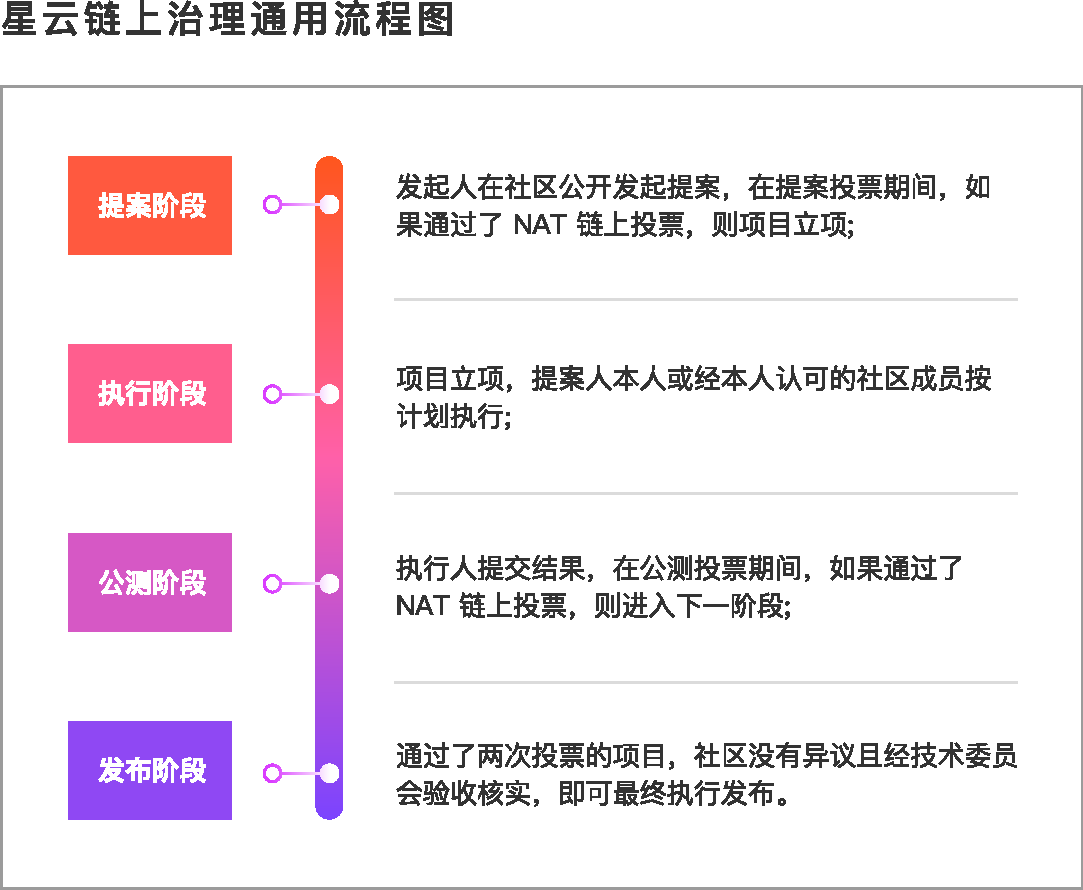
\includegraphics[width=1\textwidth]{../common/ch/on-chain-governance.pdf}
	\caption{星云链上治理通用流程图 \label{fig:on-chain-governance}}
\end{figure}

其中,“NAT链上投票”是核心手段,包括两部分:

\begin{enumerate}
	\item 投票唯一介质:NAT及其底层算法是星云链上治理的重要工具;
	\item 链上投票流程。
\end{enumerate}

本章节将对其进行重点介绍。

\subsection{投票基本原则}

星云生态通过星云主网实现链上投票。社区投出的每一票,将在星云链的区块上公开透明地展现。在星云链的系统中,投票将遵循以下基本原则:

\begin{enumerate}
	\item 投票的最基本单位是一个星云主网地址。
	\item 星云链的投票权重将参照地址的星云指数。
	\item 对系统有积极贡献的行为应被奖励更多的投票权,在投票的场景中,我们认为投票行为是对星云系统有积极贡献的行为,应被激励更多的投票权。
\end{enumerate}

\subsection{投票方式}

投票将通过星云主网上的投票智能合约实现,每个地址可以选择投赞同、反对、弃权三种票。亦可不参与投票。

\subsection{投票唯一介质:NAT}
\label{nat}

\subsubsection{概述}

\begin{itemize}
	\item \textbf{名称:} Nebulas Autonomous Token
	\item \textbf{代号:} NAT
	\item \textbf{形式:} NRC20 token
\end{itemize}

NAT是星云指数的资产形态,它以NRC20 Token的形式体现,并作为星云生态治理场景中唯一的投票介质。

\begin{center}
\fboxsep24pt
\colorbox{yellow!30}{
\begin{minipage}[c]{.8\textwidth}
	\paragraph{什么是星云指数?}
	星云指数是首个衡量区块链多维数据的价值标准,是星云核心的排序算法。

	在星云经济体中,治理的基本单位是一个\emph{地址}(参见\ref{rights})。星云指数通过对每个地址贡献度的数学表达,量化了每个“\emph{个体}”对于经济总量的贡献。星云指数分为\emph{核心星云指数}和\emph{扩展星云指数}(Extended Nebulas Ranks)。其中,核心星云指数受两个因素影响:

	\begin{enumerate}
		\item 账户在一定时期内的资产中值;
		\item 账户在一定时期内的出入度衡量。
	\end{enumerate}

	在宏观层面,核心星云指数使用经济学中经典的货币数量方程描述了区块链中货币数量、货币价值和流通速率以及生产力几者之间的关系。因此,全网的核心星云指数可以反映星云生态整体的流通性和活跃度。

	\paragraph{NAX和质押关系?}

	NAT的发行主要参考“\emph{核心星云指数}”,是核心星云指数的资产表现,NAT发行将以周为单位,参考一周之内地址的资产中值和出入度衡量计算所得的星云指数。关于星云指数的更多信息,请参考2018年6月星云研究院发布的《星云指数黄皮书》。

	\paragraph{如何查询?}

	星云指数在2019年5月6日Nebulas NOVA~\cite{nova}完成第一次投票升级后上链,可以通过Nebulas NOVA的核心能力星云区块链可执行环境(Nebulas Blockchain Runtime Environment,NBRE)实现升级。核心星云指数开源,可在线查询~\cite{CheckNR}。

\end{minipage}}
\end{center}

\subsubsection{应用场景}

NAT是星云治理中,链上投票场景的唯一介质,支持星云推进社区的治理。社区成员可以通过NAT进行链上投票表达自己对星云生态的意见,包括但不限于星云理事会的选举、星云主网通过星云区块链可执行环境(NBRE)执行星云协议表示(Nebulas Protocol Representation,NRR)、社区提案的立项、项目成果公测等。

\subsubsection{发行}
	
NAT的发行方式和比特币类似,在总量存在上限的前提下,按一定周期内全网星云指数的情况,以周为单位递减释放。

NAT协议的数量上限和星云链主网的全网星云指数值相关,释放量按周递减。递减系数为:$\lambda$。初始数值$\lambda$=0.997,即约在第180周时,发行量递减为第一周的58\%。

NAT的初始发行量以2019年5月6日星云主网Nebulas NOVA完成第一次投票升级后的全网星云指数为参照。假设全网星云指数和初始参数不变,NAT初始总量上限为1,000亿枚。

\subsubsection{管理NAT}

用户可以在NAS nano Pro~\cite{NASnano}及其他支持NRC20的客户端中~\cite{wallets}管理自己的NAT。同时,用户可以在支持星云链的区块链浏览器~\cite{explorer}上查看NAT的交易、流通情况等。

\subsection{获取NAT}

所有拥有星云主网地址的用户均有机会获得NAT。除黑名单地址外,星云主网地址的用户可以通过提升地址的星云指数、参与星云主网链上投票,或质押NAS三种方式获得NAT。


\paragraph{NAT的黑名单地址}

在NAT的发行过程中,与星云“\emph{地址}”基本权利主张(参见~\ref{rights})任何一条产生冲突的地址将被归为黑名单地址。黑名单地址只能根据其享有的权利获得部分NAT。

例如中心化交易所的地址就被归为黑名单地址。依照星云地址第一点基本权利主张,该地址具备拥有和操作星云链上资产的权利,所以交易所的归集地址可以在同等条件下按照地址的星云指数获得NAT,但这部分NAT的产权应属于对应的交易所用户。依照星云地址第二、第三点基本权利主张,在交易所证明该归集地址充分代表了相应托管资产用户提案和投票意愿之前,交易所归集地址并不具备发起提案和参与提案投票的权利,因此亦不能通过参与投票获得投票部分的NAT激励。


\subsubsection{通过提升地址的星云指数获得NAT}

对于有星云指数的地址,NAT协议将按周向该地址进行发放,发放的数量将参照该地址上一周的星云指数和星云全网星云指数的情况。

对于有星云指数的地址,每周获得NAT的数量递减,递减系数为$\lambda$。初始数值$\lambda$=0.997。

在第$i$周,获得NAT的比例约为:

\begin{align}
1\,\text{NR}=z(x_{ne},x_{e},\mu)\times\lambda^{i}\,\text{NAT}
\end{align} 

其中:
\begin{itemize}
	\item $\lambda$:衰减系数;
	\item $\mu$:投票行为的激励参数;
	\item $x_{ne}$:全网非交易所地址的星云指数总和;
	\item $x_{e}$:全网交易所地址的星云指数总和;
	\item $z(x_{ne},x_{e},\mu)$:以$x_{ne}$、$x_{e}$和$\mu$为变量的函数,星云指数和NAT的兑换比例。
\end{itemize}

\subsubsection{通过质押星云链主网原生代币(NAS)获得NAT}

从2019年5月6日开始,星云主网地址用户可以选择向投票的智能合约质押星云主网原生代币星云币(NAS)获得NAT。

质押NAS的用户将从质押开始后的第2周(即不早于2019年5月13日)开始获得NAT。如果用户取回质押的NAS,则停止获得NAT。

质押NAS的用户每周获得NAT的数量递减,递减系数为$\lambda$,初始数值$\lambda$=0.997,

第$i$周质押NAS获得NAT的比例为: 

\begin{align}
x \text{NAS} \rightarrow \alpha \times z(x_{ne},x_{e},\mu)\times g(x) \times \lambda^{i} \text{NAT}
\end{align}

其中:

\begin{itemize}
	\item $x$:质押NAS的数量;
	\item $\alpha$:质押系数,初始数值$\alpha$=5;
	\item $z(x_{ne},x_{e},\mu)$:以$x_{ne}$、$x_{e}$和$\mu$为变量的函数,星云指数和NAT的兑换比例;
	\item $g(x)$:与$x$相关的函数,用于模拟以$x$值的NAS在星云主网获得的星云指数的情况。
\end{itemize}

\vspace{2em}

\textbf{如何发起质押?} 
	
用户可以通过使用星云钱包NAS nano Pro或其他支持NAS的客户端向投票智能合约发送交易,确认要质押NAS的数量。

为了保证用户可以获得并管理NAT,用户需要用自己掌握私钥的主网地址向星云的投票智能合约发送NAS完成质押,请勿使用交易所账户发送交易。

\vspace{2em}

\textbf{如何取消质押?}

用户可以通过NAS nano Pro或其他客户端调用智能合约申请取消,取消后可立即取回质押的NAS,取消质押后,则停止获得NAT。

\subsubsection{通过参与星云链上投票获得NAT}

星云主网地址获得了NAT后,可以选择参与或不参与社区治理链上投票。在此次投票周期中,如果用户参与了投票,无论投出赞成、反对还是弃权票,均可获得投票激励。如果未参与投票,则无法获得激励。

\vspace{2em}

\textbf{激励规模}

我们认为激励的规模应该是适当的,不应该被恶意使用。投票的激励会取决于:

\begin{enumerate}
	\item 该地址当周所投NAT的数量;
	\item 该地址上一周星云指数及该星云指数对应可获得的NAT。
\end{enumerate}

当用户投出符合自己地址星云指数对应的NAT会得到激励,如果用户投出的NAT超过自己地址星云指数对应的NAT,超出部分将无法获得激励。
	
第$i$周,参与链上投票的地址获得的激励规模为:

\begin{align}
\mu\times \min\{N_{v},N_{nr}\}  \times \lambda^{i}
\end{align}

其中:

\begin{itemize}
	\item $\mu$:激励系数,初始数值$\mu$=10;
	\item $\lambda$:递减系数,初始数值$\lambda$=0.997;
	\item $N_{v}$:当周该地址投出的NAT数额;
	\item $N_{nr}$:该地址上一周的星云指数对应可获得的NAT。
\end{itemize}

即,当该地址当周投出的$N_{v}$小于或等于$N_{nr}$的时候,获得的激励数量为$\mu\times Nv$,当该地址当周投出的$N_{v}$大于$N_{nr}$的时候,获得的激励数量为$\mu\times N_{nr}$。

举例来说,假如某个地址根据上一周的星云指数值获得了10 NAT,该地址上一共有1,000 NAT,如果当周该地址投出了5 NAT,小于该地址上一周星云指数对应可获得的NAT数值(10 NAT),故将获得$10\times5=50$ NAT投票激励。如果该地址投出了1,000 NAT,超出10 NAT,则将获得$10\times10=100$ NAT投票激励。

和提升星云指数获得NAT及质押NAS获得NAT一样,通过投票激励获得的NAT也是按周递减的,递减系数为$\lambda$,初始数值$\lambda$=0.997。

\subsection{投票规则}
	
\subsubsection{投票手续费}

每次投票将收取$\theta$\% NAT将作为投票手续费,此部分手续费由星云理事会授权交由星云基金会作为NAT项目的专项运营资金管理,项目团队不得将此部分手续费直接用于投票。初始数值$\theta$=3。

\subsubsection{投票和NAT销毁}

在每个发行周期内,用户投入星云链投票智能合约的NAT将被立即销毁,销毁的比例会按照周期递减,递减速率和NAT发行的递减速率一致。每个周期内销毁部分的NAT将按照NAT销毁速率函数计算,具体公式参见附录\ref{burn}。

\subsubsection{投票通过标准}
	
投票是否通过将通过两个维度的标准来衡量:投票的参与度和赞成票的占比。

\begin{enumerate}
	\item 

	\textbf{投票参与度:}

	对于涉及到使用公共资产支持的提案,投票的参与度不得低于该提案提起资产占全网流通资产的比例。

	如某提案要求动用$X$ NAS支持,此时星云主网中流通的NAS(任何未在锁仓/质押状态、可随时在星云主网上进行转账交易的NAS)为$Y$。

	则此提案通过需要达成的全网投票参与度不得低于$X/Y$,换算成NAT来表示,及参与此次投票的NAT与该周期初期给用户的NAT的比例不得低于$X/Y$。

	对于不涉及到使用公共资产支持的提案,投票的参与度由社区共同决定,此类提案包括但不限于星云主网参数的调整、NBRE要执行的NPR等。

	\item

	\textbf{赞成票的占比:}

	在满足投票最低参与度之外,某一提案投票是否通过还需要满足赞成票占总投入票数的比例不得低于51\%。

	即假设某一提案共收到票数为N,其中赞成票为Y,反对票为N,弃权票为A,则只有当$Y/(Y+N+A) \ge 51\%$时,此提案才被视为投票通过。
\end{enumerate}

\subsection{投票监督和管理}

\subsubsection{投票流程监督}
\label{second-vote}

星云技术委员会受星云理事会委任,负责监督治理流程,保证整个流程公开透明。星云社区链上公开投票由星云技术委员会负责组织和管理。

公开投票接受社区所有成员的公开监督。针对违反星云基本权利主张的提案,星云技术委员会可以向星云理事会发起重审提案申请。星云理事会作为星云生态中治理流程正当性的监督者,有权对某一提案提起且仅能提起一次进行“\textbf{二次投票}”的要求。

当理事会提出“二次投票”的要求时,该提案被视为进入到新的投票周期进行一次新的投票。第一次投票过程中的结果不被执行,第一次投票投出的NAT不予返还,会按照当周期的烧毁速率进行烧毁。

二次投票的投票参与度需大于第一次投票的参与度。即假设第一次投票的参与度为$X/Y$,则第二次投票的参与度应大于$X/Y$,且赞成票的比例不低于51\%,方可视为投票通过。

\subsubsection{NAT参数调整}

NAT的发行过程涉及到如下系数:

\begin{enumerate}
	\item $\alpha$:质押系数,初始数值$\alpha$=5
	\item $\mu$:投票奖励系数,初始数值$\mu$=10
	\item $\lambda$:递减系数,初始数值$\lambda$=0.997
	\item $\theta$:投票手续费,初始数值$\theta$=3
\end{enumerate}

系数的调整需要经过星云生态的治理投票流程,星云基金会或NAT项目团队无权擅自调整系数。





\newpage
\bibliography{reference}

\newpage
\begin{appendices}
\section{Nebulas Autonomous Token NAT issuance algorithm}

The issuance of NAT is based on each user's Nebulas Rank, voting behavior, and pledge amount.

\subsection{Overview}
The issuance of NAT is performed according to the weekly calculation cycle of Nebulas Rank (note: voting periods and Nebulas Rank calculations utilize the same weekly period). Based on these weekly cycles, NAT distribution is executed for each address on Nebulas looking at voting behavior, pledging and the previous week Nebulas Rank score.

Detailed explanation:
For the period $i$, the new NATs $\mathcal{T}_i$ in the system is divided into three parts - the NR part: $\mathcal{A}_i$, the voting incentives part: $\mathcal{V}_i$, the pledge part: $\mathcal{D}_i$.
In addition, NATs used for voting will be burned/destroyed with respect to certain percentage. Assuming that for the cycle $i$, the reduced amount of NATs on the network (due to voting) is $\mathcal{M}_i$, then the total amount of NATs in the system is:
\begin{align}
\sum_{i=1}^{\infty} (\mathcal{A}_i + \mathcal{V}_i + \mathcal{D}_i - \mathcal{M}_i)
\end{align}

For convenience, all symbols used in this section and their corresponding explanations are listed below:
\begin{itemize}
\item $\mathcal{C}_i$: The sum of Nebulas Rank scores in the system in  cycle $i$;
\item $c_{i,j}$: User $j \in \mathcal{U}$'s Nebulas Rank Score in cycle $j$ ;
\item $d_{i,j}$: User $j \in \mathcal{U}$'s total amount of pledged NAS in cycle $i$;
\item $v_{i,j}$: User $j \in \mathcal{U}$ 's total amount of voted NATs in cycle $i$.
\end{itemize}

\subsection{NR part}
This part is related to the user's Nebulas Rank score, defined by
\begin{align}
    f(x) = g(x)\lambda^i
\end{align}
\noindent where $x$ is the user's Nebulas Rank score; $g(x)$ is a proportional function that adjusts the relationship between NAT and the Nebulas Rank and satisfies $g(0) = 0$ ;$\lambda$ is the attenuation coefficient, and $\lambda < 1$.
Since $\lambda < 1$, it is easy to know $\lim_{i\to \infty}f(x) = 0$.

The total amount of this part  in cycle $i$ is:
\begin{align}
\mathcal{A}_i = \sum_{i=1}^{\infty}f(\mathcal{C}_i).
\end{align}

\subsection{Voting incentives part}
The voting incentives part are related to users' voting behaviors and their Nebulas Ranks. For user $j \in \mathcal{U}$, the voting incentives part are defined by :
\begin{align}
\mu f(x_{i-1,j}) \min\{\frac{v_{i,j}}{f(x_{i-1,j})},1\}
\end{align}
\noindent where $\mu$ is the voting incentive coefficient, $\mu > 1$, which means that the user's voting behavior is encouraged by additional rewards, which can be adjusted according to the amount of circulating NAS in the system.

\subsection{Pledge part}
The pledge part of NATs should be related to the NR part obtained based on the users‘ improved Nebulas Rank. Based on the property of Nebulas Rank, for a given amout of a user's NAS, there is an upper bound of his Nebulas Rank score $h(d_{i,j})$~\cite{ImproveNR},

So, we define the NAT obtained by the pledge part to be:
\begin{align}
\mathcal{D}_i = \sum_{i=1}^{\infty}\alpha f(h(d_{i,j}))
\end{align}
\noindent where $\alpha$ is the pledge incentive coefficient.


\subsection{Destroyed/Burned Part}
\label{burn}
Each time a address votes using NAT, all NAT used is immediately burned and is no longer usable. However, NAS is distributed by 3 methods; as explained earlier, they are: NR part, voting incentives part, and pledge part. Therefore, we can state that while NAT is burned, NAT is also redistributed to the network weekly and has a network burn rate. In addition, the Nebulas Council charges a fee of $\theta\%$ for each vote in order to pay for the necessary expenses of maintaining the voting services. Therefore for each user, define the destroyed part to be\begin{align}
(1-\theta\%) \times \beta^i \times v_{i,j}
\end{align}
\noindent where $\beta$ is the destruction coefficient and $\beta < 1$. therefore,
\begin{align}
    \mathcal{M}_i = \sum_{i=1}^{\infty} (1-\theta\%) \times \beta^i \times v_{i,j} .
\end{align}

\subsection{Analysis}

note:
\begin{itemize}
\item The current version tentatively agrees that there is no difference between a vote and a negative vote, that is, their return ratios are equivalent. It can then be set according to the ticket's type and multiplied by a different return coefficient $\mu_1$;
\item Considering the change of the total Nebulas Rank in the system after the vote is completed, a coefficient $\mu_2$ can be multiplied to reflect the status of the system.
\end{itemize}

\begin{property}
	The algorithm satisfies the convergence of the total amount of NAT; in return, the total amount of NATs does not exceed the upper bound at any time.
\end{property}

\begin{proof}
	According to the details within the Nebulas Technical White Paper, the fixed total amount of NAS is $10^9$ with an average weekly issuance amount (on the basis of the fixed total) of $0.2\%$; in return, the total amount of NAS existing on the market for the $n$ cycle will not exceed $10^9 (1+0.002n) $

	Next, we prove that the sum of all median values of assets of all addresses in one cycle (as defined in the Nebulas Rank Yellow Paper) does not exceed the total amount of existing NAS on the market. This is because for any NAS asset with quantity $y$,it can appear for half of the period (three and a half days) in only one address, so it can at most contribute $y$ to the sum of all median values of assets of all addresses.

	Also according to the Nebula Rank Yellow Paper, the Nebulas Rank score of any
	single address can not not exceed the median value of assets of that address
	(for the same period; note that Nebulas Rank and NAT calculations are weekly
	and synchronized). That is because in the formula $\Omega(\cdot)\Psi(\cdot)$
	for calculating the Nebulas Rank, the Wilbur function $\Omega(\cdot)$, whose
	input is the median value of the asset, satisfies $\Omega (x) \leq x$, and
	the value of the in-and-out function $\Psi(\cdot)$ does not exceed 1.

	Combined with conclusions above, in cycle $n$, the sum of Nebulas Rank scores of all addresses does not exceed $10^9(1+0.002n)$, so that the NR part does not exceed $g(10^9(1+0.002n)))\lambda^n$.

	Also, since the NAT of the voting incentive part does not exceed the NR part multiplied by $\mu$, even if the returned NATs from voting is added, the total increment of NAT in voting incentive part in cycle $n$ does not exceeds $\mu g(10^9( 1+0.002n))\lambda^n$. In addition, the increment NAT from the pledge port does not exceed the total amount of NAS $g (10^9(1+0.002n))\lambda^n$.

	Finally, to prove the convergence of the total amount of NAT, since NATS  from the NR part, the pledge part and the incentive part are exponentially decayed with time, it is only necessary to prove the series
	\begin{align}
	\sum_{n=1}^{\infty} \mu g(10^9(1+0.002n))\lambda^n
	\end{align}
    are	convergence. Since $g(\cdot)$ is a linear function,
	\begin{align}
	\lim_{n\rightarrow \infty} \frac{\mu g(10^9(1+0.002(n+1)))\lambda^{n+1}}{\mu g(10^9(1+ 0.002n))\lambda^n} = \lambda <1
	\end{align}
	The onvergence of the series can be obtained by the ratio test.
\end{proof}

The series can be convergent and verified by the comparison method.

Moreover, the above voting algorithm has the following positive properties.
\begin{enumerate}
	\item \textbf{Anti-snowball effect:} If we always return NATs  with respect to fixed ratio, a user can vote all his  NAT to enjoy a return ratio greater than 1 (such as 1.1); then his total amount of  NATs will be exponentially increasing, as  $1.1^n$
	\item \textbf{Anti-bribe:} If a user with a low Nebulas Rank buys a large amount of NAT to vote, since the corresponding $x_{i-1}^j$ are small for addresses with a low Nebulas Rank score, very few NATs are returned while most of them are burned. It causes the user loses many NATs as penalization.
	\item \textbf{Anti-inflation:} The depreciation of NAT can be effectively controlled because the issuance of NATs is related to the total amount of NAT in the current market.
	\item \textbf{Head-effect:} A user with a high Nebulas Rank during the early stages can have a higher total amount of NATs.
\end{enumerate}

\section{Nebulas Asset Supervision}

\label{supervision}

As show in Figure~\ref{fig:assets}, Nebulas assets include two parts: Community public assets and Nebulas Foundation assets.

\subsection{Community public assets}

\subsubsection{Composition}

\begin{itemize}
	\item 35,000,000 NAS (35\% of total circulation): community reserved assets as stated in the \textit{Nebulas Non-technical Whitepaper}
    \item 8,219.1744 NAS/Day: from consensus/block generation issuance, includes:
	    \begin{itemize}
			\item 2\%: Consensus/block generation issuance
			\item 1\%: Nebulas Council Project Development Fund reserve
		\end{itemize}
	\item 1\%(initial): Native incentive for Developer Incentive Protocol (DIP)~\cite{mauvepaper}, since May 13, 2019
\end{itemize}

\subsubsection{Supervision}

Public assets belong to the Nebulas community; they are automatically distributed and managed via the on-chain governance process and is overseen by the Nebulas Council.

\subsection{Nebulas Foundation assets}

\subsubsection{Composition}

\begin{itemize}
	\item 20,000,000 NAS (20\%): Nebulas team reserved as stated in the \textit{Nebulas Non-technical Whitepaper}
    \item 5,000,000 NAS (5\%): Nebulas Community Development Fund (Eco-investment Balance)
	\item Early private equity project development funds
	\item Early ecological investment income
\end{itemize}

\subsubsection{Supervision}

The Nebulas Foundation assets are managed by the Nebulas Foundation. The Foundation shall ensure that the use of asset information is open and transparent.

\begin{figure}
	\centering
	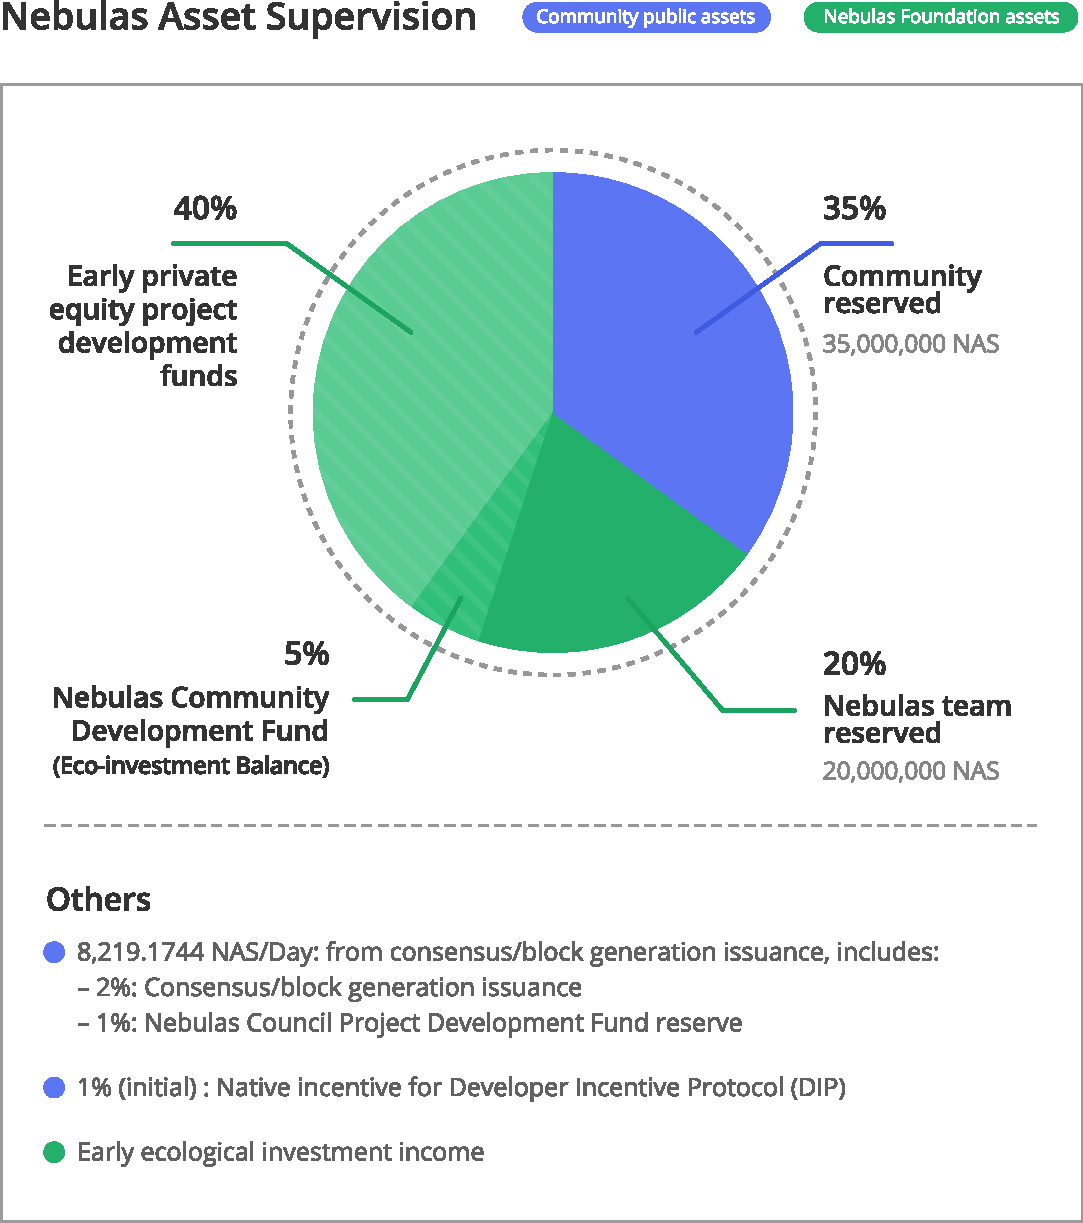
\includegraphics[width=1\textwidth]{../common/en/assets.pdf}
	\caption{Nebulas Assets Supervision \label{fig:assets}}
\end{figure}
\newpage
\section{Change Log}
\begin{itemize}
\item{0.0.1} Release. 2019.8
\item{0.0.2} Release. 2019.11
\end{itemize}

\end{appendices}

\end{document}
